\section{Stoke relations}
\label{sec:StokeRel}

In this section the Stoke relations and the associated presumptions about the 
material system are discussed. 

To get to the Stoke relations, we have to start from a system with two materials of different 
refractive indexes $n_1$ and $n_2$. When rewriting the reflected and transmitted partial amplitudes through the initial
amplitude $E_{0}$ and applying invariance in regards to time as depicted in Figure \ref{fig:Stokrel}, we reach the a set of equations

\begin{gather}
    t(\theta_1)t'(\theta_2) = 1 - r^2(\theta_1)\\
    r'(\theta_2) = -r (\theta_1) \label{eq:StokeRel2}
\end{gather}

that are called \textbf{Stoke relations}\mycite{Hecht.2005}. 

The fundamental message of the Stokes relation is on the one hand the relation between the reflection and the transmission 
coefficient and further a phase relation at the boundary surface. Equation \ref{eq:StokeRel2} states that the  waves on the two sides 
of the spectrum have got a phase difference of $\pi$.

\begin{figure}[ht]
    \centering
    \begin{subfigure}[b]{0.3\textwidth}
        \centering
        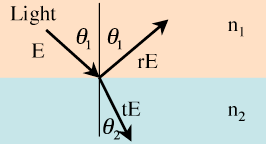
\includegraphics[width = \textwidth]{Bilder/Grundlagen/StokeRelat1.png}
        \caption{Forwards in time}
        \label{fig:Stokfor}
    \end{subfigure}
    \hfill
    \begin{subfigure}[b]{0.3\textwidth}
        \centering
        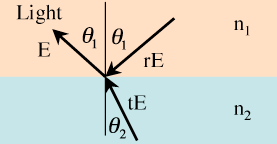
\includegraphics[width=\textwidth]{Bilder/Grundlagen/StokeRelat2.png}
        \caption{Backwards in time}
        \label{fig:Stockback}
    \end{subfigure}
    \hfill
    \begin{subfigure}[b]{0.3\textwidth}
        \centering
        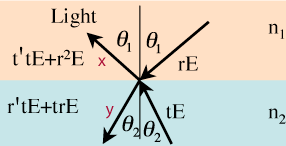
\includegraphics[width=\textwidth]{Bilder/Grundlagen/StokeRelat3.png}
        \caption{\ref{fig:Stockback} with all possible fields}
        \label{fig:five over x}
    \end{subfigure}
       \caption{Stokes' treatment of reflection and refraction}
       \label{fig:Stokrel}
\end{figure}

To arrive at those relations we used \textit{time reversal symmetry}. The \textit{T-invariant} can only be applied to a system in which the process is physically "allowed"
for the inverted situation. In this case, it means that there is no absorption in this system.